\section{Satisfiability}
\label{sec:sat}
The Boolean Satisfiability (SAT) problem attempts to determine if there exists a total truth assignment to a given propositional formula, that evaluates to $true$. Generally, a propositional formula is any combination of the disjunction and conjunction of literals (as an example, $a$ and $\neg a$ are literals). For example, the proposition $a \land b$ is satisfiable; when $a$ and $b$ are assigned to $true$, the formula is satisfied.  On the other hand, the proposition $a \land \neg a$ is unsatisfiable; no such assignment can be found to satisfy both $a$ and $\neg a$. SAT solvers in work over a constraint system of propositional logic to determine satisfiability. Satisfiability Modulo Theories (SMT) solvers also address the SAT problem, but can work over propositional logic or predicate logic with quantifiers. An SMT solver works over a conjunction of literals, as is the case with SAT solvers, but the literals can be expressed as predicates over non-boolean variables, such as $x > 0$. A boolean literal can be satisfied with a finite number of possible assignments; this is not always the case with SMT formula.

\subsection{UNSAT Cores and Minimal Unsatisfiable Subsets}
A constraint system $C$ is an ordered set of $n$ abstract constraints $\{C_1, C_2, ..., C_n\}$ over a set of variables. The constraint $C_i$ restricts the allowed assignments of these variables in some way~\cite{liffiton2016fast}. Given a constraint system, we require some method of determining, for any subset $S \subseteq C$, whether $S$ is \textit{satisfiable} (SAT) or \textit{unsatisfiable} (UNSAT). Given a constraint system $C$, there are certain subsets of $C$ that are of interest in terms of satisfiability. %Definitions 2-4 are taken from research by Liffiton et. al.~\cite{liffiton2016fast}. 

For a given unsatisfiable problem, SAT solvers (and SMT solvers) attempt to provide proof of unsatisfiability by providing a subset of UNSAT clauses known as \textit{UNSAT cores}. In general, this is useful information to have regarding the constraint system in question. 

\begin{definition} A Minimal Unsatisfiable Subset (MUS) $M$ of a finite constraint system $C$ is a subset $M \subseteq C$ such that $M$ is unsatisfiable and $\forall c \in M$ : $M \setminus \{c\}$ is satisfiable. 
\end{definition}

\begin{definition} UNSAT core: Let $C$ be a finite set of constraints and $U \subseteq C$ an unsatisfiable subset. A constraint $c \in U$ is an UNSAT core for $U$ if $U \setminus \{c\}$ is satisfiable. A set of all unsatisfiability cores of $U$ constitute an MUS for $C$. 
\end{definition}

Intuitively, an MUS is the minimal explanation of the constraint systems infeasability and the UNSAT cores are the building blocks of the MUS. In recent years, a number of efficient algorithms have been introduced to find MUSs~\cite{liffiton2005max} and most of them focus on finding a single such subset~\cite{belov2012towards, belov2013core, belov2012muser2}. More recently, algorithms have been introduced that can find all such minimal unsatisfiable subsets~\cite{GhassabaniGW16, Ghassabani2017EfficientGO,bendik2018online}. 

\subsection{Inductive Validity Cores} Given a complex model, it is useful to extract traceability information related to the proof; in other words, which elements of the model were necessary to construct the proof. An algorithm was introduced by Ghassabani et al. to provide Inductive Validity Cores (IVC) as a way to determine which model elements are necessary for the inductive proofs of the safety properties for sequential systems~\cite{GhassabaniGW16}. Given a safety property of the system, a model checker is invoked to construct a proof of the property. The IVC generation algorithm extracts traceability information from the proof process and returns a minimal set of the model elements required in order to prove the property. Later research extended this algorithm in order to produce all minimal IVC elements (\aivcalg)~\cite{Ghassabani2017EfficientGO,bendik2018online}. 

The \aivcalg algorithm considers a constraint system consisting of the assumptions and contracts of system components and the negation of the safety property of interest (i.e. the top level event). It then collects all Minimal Unsatisfiable Subsets (MUSs) of this constraint system; these are the minimal explanations of the constraint systems infeasibility in terms of the \textit{negation} of the safety property. Equivalently, these are the minimal model elements necessary to prove the safety property. 

\subsection{Ordered Binary Decision Diagrams}
A Binary Decision Diagram (BDD) is a data structure used to encode Boolean formulae.
\begin{figure}[!htb]
        \center{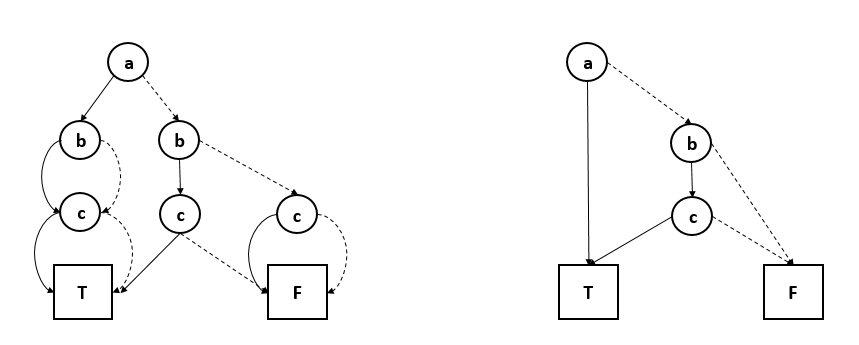
\includegraphics[width=0.8\textwidth] {images/bdd.png}}
        \caption{\label{fig:bdd} Binary Decision Diagrams of the Formula $a \lor (b \land c)$}
\end{figure}
As shown in Figure~\ref{fig:bdd}, it is a rooted, directed, acyclic graph with internal decision nodes and two terminal nodes (\textit{true} and \textit{false}). Each of the decision nodes is labeled with a Boolean variable and has two child nodes, low child and high child. The edge from a node to its low child represents the assignment of \textit{false}, likewise the edge to the high child represents the assignment of \textit{true}. The BDD is called \textit{ordered} if different variables appear in the same order on all paths from the root. Intuitively, following a path from the root to the \textit{true} terminal node represents a valid assignment to the Boolean formula (invalid in the case of ending on the \textit{false} terminal node). 

BDDs can also be reduced by the removal of isomorphic subgraphs. The BDD shown on the right of Figure~\ref{fig:bdd} is the reduced form of the BDD on the left. 











